%---------------------------------------------------------------------
% This is a sample file for the jotarticle class.
%
% (c) Susanne Cech, Departement Informatik, ETH Zuerich, 
%     susanne.cech@inf.ethz.ch, 2003-02-27
%
%---------------------------------------------------------------------
% last change: 2003-02-27
%---------------------------------------------------------------------

\documentclass{jotarticle}

%---------------------------------------------------------------------
% GENERAL INFORMATION
%---------------------------------------------------------------------
% This template is to be used for JOT-articles only.
%
% Read this documentation carefully, it will simplify your work.
% Some commands are to be used out by the authors, some by the JOT
% team only. I've tagged the commands with [AUTHOR] and [JOT].
%
% To compile your LaTeX-document, I suggest using pdflatex. We will
% use it here as well because it generates directly PDF, thus 
% a clickable document with internal and external links (HTML) is 
% the result.
%
% Please note: When using pdflatex, your picture files need to be
% either in PNG or PDF-format. 
%
% I'm happy about every comment. If you have questions, suggestions,
% comments, etc, please send me an email: susanne.cech@inf.ethz.ch
%---------------------------------------------------------------------


%---------------------------------------------------------------------
% CONFIGURATION
%---------------------------------------------------------------------
% There are two parts configuration parts. The author can enter the 
% first part, that is information regarding the author and the 
% article.
% The second part is to be filled out by the JOT team. Authors please
% leave it as it is, as any non-suitable input will be removed.
%---------------------------------------------------------------------


\newenvironment{mylisting}
{\begin{list}{}{\setlength{\leftmargin}{1em}}\item\scriptsize\bfseries}
{\end{list}}

\newenvironment{mytinylisting}
{\begin{list}{}{\setlength{\leftmargin}{1em}}\item\tiny\bfseries}
{\end{list}}


%---------------------------------------------------------------------
% CONFIGURATION: BY THE AUTHOR
%---------------------------------------------------------------------
% [AUTHOR] Add the title of your article here
%---------------------------------------------------------------------
\title{A Tool for Supporting and Automating the Development of Component-based Embedded Systems} %A Tool for Supporting the Development of Component-based Embedded Systems}
%---------------------------------------------------------------------
% [AUTHOR] Add the authors here
%          Several authors can be separated by either \\ or \and
%          Use bold font for the authors name as shown in the example.
%---------------------------------------------------------------------
\author{\textbf{Rafael L. Cancian, Marcelo R. Stemmer}, Departement of Eletrical Engineering, 
        Federal University of Santa Catarina\\
        \textbf{Alexandre Schulter, Ant\^{o}nio A. M. Fr\"{o}hlich}, Departement of Computer Science, 
        Federal University of Santa Catarina\\
}
%---------------------------------------------------------------------


%---------------------------------------------------------------------
% CONFIGURATION: BY THE JOT TEAM
%---------------------------------------------------------------------
% [JOT] Set first page and last page of the article/column
%---------------------------------------------------------------------
\firstpage{1}
\lastpage{22}
%---------------------------------------------------------------------
% [JOT] Enter the volume and number of the issue. 
%       Here: vol 2, no 3
%---------------------------------------------------------------------
\jotvolume{1}
\jotnumber{1}
%---------------------------------------------------------------------
% [JOT] Enter the month and year when the issues is published.
%       Here: March 2003
%---------------------------------------------------------------------
\jotmonth{8}
\jotyear{2007}
%---------------------------------------------------------------------
% [JOT] [OPTIONAL] Enter how to cite this article 
%       This is generated. In case it does not fit your expectations,
%       you can enter it yourself.
%---------------------------------------------------------------------
\howtocite{\href{http://www.jot.fm/general/JOT_template_LaTeX.tgz}%
{http://www.jot.fm/general/JOT\_template\_LaTeX.tgz}}
%---------------------------------------------------------------------
% [JOT] Set type of paper, i.e. column or article
%       This is needed for the generation of \howtocite
%---------------------------------------------------------------------
\papertype{document}
%---------------------------------------------------------------------
% [JOT] Set the filename. 
%       This is needed for the generation of \howtocite
%---------------------------------------------------------------------
\filename{tools2007}
%---------------------------------------------------------------------
% [JOT] Enter the names of the authors as comma-separated list.
%       This is needed for the generation of \howtocite.
%       (I know this is ugly -- I will work on that as soon as type
%       permits it.) 
%---------------------------------------------------------------------
\authornames{Alexandre Schulter, Rafael L. Cancian, Marcelo R. Stemmer, Ant\^{o}nio A. M. Fr\"{o}hlich}
%---------------------------------------------------------------------


%---------------------------------------------------------------------
% START OF THE DOCUMENT
%---------------------------------------------------------------------
% This is where the document starts. In this example, I will guide
% you through this sample article with the explanation of possible
% commands you should use.
%---------------------------------------------------------------------


%---------------------------------------------------------------------
\begin{document}
%---------------------------------------------------------------------

%---------------------------------------------------------------------
% ABSTRACT
%---------------------------------------------------------------------
% [AUTHOR] Clearly a job for the author :-)
%          Add your abstract here
%---------------------------------------------------------------------
\begin{abstract}
% contextualização e problemática
%Sistemas computacionais embarcados são compostos por hardware e software e geralmente executam aplicações específicas em ambientes altamente restritos. Por isso, tanto o suporte de software quanto o de hardware devem ser mínimos e adaptados aos requisitos da aplicação. A crescente complexidade dos sistemas embarcados e as restrições cada vez mais fortes de diminuição do tempo de desenvolvimento, redução dos custos de engenharia, além das tradicionais restrições de capacidade de memória, acesso a dispositivos e poder de processamento, têm exigido novas abordagens, metodologias e ferramentas para seu desenvolvimento. Em geral, nesse domínio, são indispensáveis o reuso de componentes, transparência arquitetural, overhead mínimo, e facilidades de configuração e composição do sistema.
% abordagem adotada
%A metodologia Application Oriented System Design (AOSD) foi criada para tratar essas questões, e visa guiar o desenvolvimento de sistemas embarcadados que atendam exatamente os requisitos da aplicação, gerando um suporte mínimo. Essa metologia propõe uma boa combinação de técnicas de orientação a objetos para a análise do domínio dos sistemas embarcados, a separação de aspectos funcionais e não-funcionais para prover reuso e transparência arquitetural, algumas técnicas de implementação (como metaprogramação estática) para evitar overhead, e um conjunto de ferramentas de suporte para a configuração e geração semi-automática do sistema embarcado (aplicação, suporte de software e plataforma de hardware).
% contribuições
%Este artigo foca na estrutura e desenvolvimento das ferramentas de suporte, que têm sido usadas com sucesso para a configuração e geração do EPOS (Embedded and Parallel Operating System), criado a partir da AOSD. Essas ferramentas recebem como entrada o código-fonte de uma aplicação (que utiliza a API do EPOS) e, com poucos cliques do mouse sobre a interface gráfica, gera a imagem completa do software e, no caso de hardware reconfigurável, também o arquivo de configuração da FPGA. Esse artigo mostra ainda que, pelo modo como as ferramentas foram concebidas, elas têm uma grande abrangência, e poderiam ser usadas com sucesso para configurar e gerar diversos outros sistemas.
% resultados conseguidos
%Com o desenvolvimento dessas ferramentas, foi possível configurar e gerar de forma semi-automática (ou totalmente automática em alguns casos) várias instâncias de sistemas embarcados para diversas arquiteturas (AVR, MIPS, SparcV8, PPC405, Intel32) de forma rápida e fácil. Para ilustrar esse processo e o uso das ferramentas, este artigo mostra como estudo de caso a geração de um sistema embarcado para suporte a uma aplicação simples de decodificação de áudio e os resultados obtidos.
Embedded systems are comprised of hardware and software and usually run dedicated applications in environments with highly restricted resources, such as memory constrained devices, microcontrollers with low processing power, and wireless sensors running on batteries. These systems must exactly match applications' requirements, with minimum support. The growth in application complexity and even more strong constraints demand new approaches, methodologies, and tools to assist embedded systems development. Usually, in this domain, reuse of components, architectural transparency, low overhead, and reconfigurability are essential features. The Application-Oriented System Design (AOSD) method was created to deal with these issues, and aims at guiding the development of embedded systems that exactly match application requirements. To deliver each application a tailored run-time support system calls for a good combination of object oriented techniques, the separation of functional and non-functional aspects, some implementation techniques, and a sophisticated tool that helps the developer in managing component configurations and automating the generation of embedded systems.

This paper describes a configuration and system generation tool that is being successfully used with EPOS (Embedded and Parallel Operating System), an OS developed using AOSD. This tool receives the application source-code (using EPOS API) as input and, after a few mouse clicks, builds the entire computational support, comprised by software and, if hardware is reconfigurable, the FPGA configuration file. This paper also shows that the design of these tools allows them to be used for configuring and building several other systems, not only EPOS. The development of this tool enabled the configuration and generation of several embedded systems instances for several different architectures in an automatic way. To illustrate this process and the tool's usage, this paper describes a case study of the generation of an embedded system that supports a simple audio decoder application.

\end{abstract}
%---------------------------------------------------------------------


%---------------------------------------------------------------------
%%%%%%%%%%%%%%%%%%%%%%%%%%%%%%%%%%%%%%%%%%%%%%%%%%%%%%%%%%%%%%%%%%%%%%%%%%%%%%%
\section{Introduction}
%%%%%%%%%%%%%%%%%%%%%%%%%%%%%%%%%%%%%%%%%%%%%%%%%%%%%%%%%%%%%%%%%%%%%%%%%%%%%%%

%The success in the development of embedded systems depends on aspects such as low cost, quickness to market and cost-effective variations in the product. Component-based technology is being used in other fields to reach these objectives, since it provides the basis for software reuse and adaptability. 
%High performance mobile and embedded applications, such as wireless monitoring sensors, ..., and ...  need run-time support systems providing basic functions(???). The time required to develop such applications is sometimes severely impacted (frequently impacted?) by the time required to develop and/or optimize their support systems. Although embedded systems are becoming more and more complex, there is no room in this extremely competitive sector for development strategies that incur in extended time-to-market.
%Automation of parts of the development process is desirable... There exists a demand for this...

Embedded systems are being extensively used in several industrial sectors as an effective alternative to control machines, automobiles, domestic appliances, personal gadgets, and virtually every device that includes electronic components. Recent statistics reveal that over 99\% of the microprocessors produced nowadays are used in embedded systems and that in 2005 the number of embedded systems in the planet rose above the number of humans \cite{pop2005}. Besides growing in number, these embedded systems are also becoming more and more complex as they benefit from microchip advances.

In this context, the System-on-a-Chip (SoC) approach emerges as a compromise between complexity and cost. Programmable Logic Devices (PLD) enable developers to evaluate complex designs in short periods of time by applying techniques that are closer to software development than to traditional hardware development. Getting a SoC out off a Field-Programmable Gate Array (FPGA), however, is not a trivial task and requires an intricate engineering process. From the hardware perspective, much effort has been put in tools that assist designers in selecting and configuring hardware components, or Intellectual Property (IP) blocks, and also in generating the necessary glue logic. Indeed, some embedded systems can be completely implemented in hardware with this approach. Nonetheless, the more complex the application is, greater is the probability it will need some sort of run-time system to adequately support its execution on top of a (soft-core) processor.

From the software perspective, this research group has been exploring methodologies and tools to sustain the development of embedded systems as aggregates of reusable components. One of the main challenges surmounted along this long-term research concerns architectural transparency for the run-time support system. In the realm of embedded systems, run-time support must often be provided under distinct architectures. For instance, an application running on a simple 8-bit microcontroller will probably be supported by a run-time library, while a multitask application running on a 32-bit microprocessor will probably require a microkernel. In order to enable application portability, a component-based embedded system must present the same interface in both cases. Indeed, the component should be the same, since its interface and behavior remains the same; only the software architecture is different. Our approach has so far enabled the development of run-time support systems whose architecture can be defined according to particular application needs.

Embedded applications usually don't find adequate run-time support on all-purpose operating systems and hardware. Application-Oriented System Design (AOSD) is an useful solution for this kind of applications, as demonstrated in previous works \cite{Frohlich2001} \cite{Frohlich2000} \cite{Polpeta2004} \cite{Santos2006}. Application-Oriented Operating Systems (AOOS) are targeted towards the applications, which means they are composed only from selected software components that are adapted to finely fulfill application requirements. Additionally, an AOOS may be supported by a hardware platform created by the composition and synthesis of proper hardware components. Delivering each application a tailored run-time support system, besides requiring a comprehensive set of well-designed software and hardware components, also calls for a sophisticated tool that will help the developer in creating component configurations, a task that includes the identification, selection, configuration, adaptation, and composition of those components.

In this work we present an approach to the configuration management of component-based embedded systems which enables partial automation of the development process of mobile and embedded applications, contributing to an increase in productivity. Also, the ability to easily generate optimized versions of an operating system and a hardware platform for each of the applications that are going to use is of great value in the domain of high performance embedded computing, since it results in performance gains and resource usage optimization.

%Scope of the contribution: a set of functionalities for a tool that supports developers in identifying, selecting, configuring, adapting, and composing software and hardware components for the generation of instances of application-oriented operating systems and underlying hardware.

This paper is organized as follows: %Section \ref{sec:relatedwork} shows some approaches and tools for developing embedded systems. 
Section \ref{sec:AOSD} briefly describes AOSD, our approach to the design of component-based embedded systems. Section \ref{sec:concepts} presents the main concepts and structure of a tool that is able to configure and generate embedded systems. Section~{\ref{sec:implementation}} describes the details of a prototype implementation. Section \ref{sec:casestudy} presents a case study that demonstrates the use of this tool and the last section presents some conclusions and a road map for future work.
%Such approach is described in terms of a component description language, a set of functionalities for a conceptual tool and, subsequently, a prototype implementation. We then show how this tool improves development processes by presenting a case study involving a real application.


%%%%%%%%%%%%%%%%%%%%%%%%%%%%%%%%%%%%%%%%%%%%%%%%%%%%%%%%%%%%%%%%%%%%%%%%%%%%%%%
%\section{Related Work}
%\label{sec:relatedwork}
%%%%%%%%%%%%%%%%%%%%%%%%%%%%%%%%%%%%%%%%%%%%%%%%%%%%%%%%%%%%%%%%%%%%%%%%%%%%%%%

% IDÉIA PRINCIPAL DO PARÁGRAFO: reapresentar o escopo do trabalho dando a linha pela qual serão apresentados trabalhos relacioandos (talvez deva ficar na introdução)
% INTRODUÇÃO AO TEXTO:
% RASCUNHO DO CORPO DO PARÁGRAFO: Sistemas embarcados são compostos de componentes de hardware e software. Componentes devem ser independetes de arquitetura e reusáveis. A composição exige análise do cenário de execução e conhecimento da arquitetura-alvo para exploração do expaço de projeto. ...
% CONCLUSÃO DO PARÁGRAFO:
% REFERÊNCIAS A CITAR:

%Embedded Systems have grown hugely in number and complexity in the last decades.  Despite this growth, “the state-of-art in software engineering for embedded systems is far behind other application areas” and “composition of embedded systems software still has a long way to go to reach that level” \cite{gensler2001}. To reach it, many methodologies and approaches were proposed, and “actually, component-based software engineering is becoming a mainstream approach to embedded systems development” \cite{shang2002}. Although the common sense of developing reusable components in software development, given the several steps, models and views in an embedded system project, “due to the lack of a common modeling framework for embedded software design, extracting information from one model for use in another has to be a manual process, and thus incurs high cost, limiting the benefits of model-based approach”, and one of the main unsolved problems is ”to develop a method that supports information flow from one model to another” \cite{shang2002}.

% IDÉIA PRINCIPAL DO PARÁGRAFO: apresentar técnicas de co-design e geraÇão de SoCs
% INTRODUÇÃO AO TEXTO:
% RASCUNHO DO CORPO DO PARÁGRAFO: 
% CONCLUSÃO DO PARÁGRAFO:
% REFERÊNCIAS A CITAR:Givargis, vincenteli, SystemC

%Regarding the hardware platform, technological advances allowed for the production of larger, faster, and cheaper FPGAs. Along with the pressure to reduce the time-to-market and non-recurring engineering costs of embedded systems, these advances are making FPGAs an interesting alternative for several industrial projects \cite{mei2000}.  Moreover, they facilitate the development of embedded systems as hardware-software co-design projects implemented as Systems-On-a-Chip (SoC). In this context there have been many contributions that promoted significant advances in the development of PLDs as a SoC for embedded applications. A first issue was the development of Intellectual Properties (IPs) as reusable hardware components (cores). “Intellectual Property (IP) reuse is one of the most promising techniques addressing the design complexity problem. IP reuse assumes that pre-designed components can be integrated into the design under development, thereby reducing design complexity and time.” \cite{zhang2001}.

%An approach to generate SoCs is the Platform-Based Project, with generation of IPs and processors you synthesized, as Leon2, OpenRisc and Nios \cite{mattsson2004}.  This approach really promoted significant advances, but the produced platforms are not sufficiently configurable to really adapt themselves to the application’s requirements. Therefore it seems like only grouping in a single chip the diverse physical components that would compose embedded systems in distinct chips (processing, devices, memory).  This approach synthesizes only the necessary components to the application, but usually the components themselves are not adaptable. Indeed, only partial pieces are configurable, as the communication system \cite{pasricha2004}, and that's usually done by the developer, but not by automated tools.

%Other approach that targets the automatic generation of SoCs based on the application is the partitioning supported by specific languages or libraries, like SystemC (http://www.systemc.org), CynApps (http://cynapps.com), CoWare (http://www.coware.com) and SpecC (http://www.cecs.uci.edu/specc). This approach may be interesting for many reasons, though some questions, as the need of identifying in the code wide functional blocks that can be combined in synthesizable components is still a great challenge for current compilers. Also synchronous languages, a group of languages proposed for automatic synthesis of embedded software \cite{Berry1991}. With this model of computation, the designers can specify their designs with minimal implied implementation attributes. While very powerful, synchronous languages support a model of computation that restricts the design space considerably because of the synchronous communication hypothesis \cite {Hsieh1999}.

% IDÉIA PRINCIPAL DO PARÁGRAFO: Apresentar e discutir alguns trabalhos sobre composição de componentes e configuração de sistemas, enfatizando aspectos em comum com este trabalho
% INTRODUÇÃO AO TEXTO:
% RASCUNHO DO CORPO DO PARÁGRAFO: PURE?, Flux OSkit?, Knit?, more recent (2006-2007) references, Linux package selector (not that much related?), VHDL tools?, ... note: obviously none of them feature AOOS generation, but does any of them at all support the development of component-based embedded systems?
% CONCLUSÃO DO PARÁGRAFO:
% REFERÊNCIAS A CITAR:



% IDÉIA PRINCIPAL DO PARÁGRAFO: Apresentar e discutir alguns trabalhos sobre exploraçao do espaço de projeto, enfatizando aspectos em comum com este trabalho
% INTRODUÇÃO AO TEXTO:
% RASCUNHO DO CORPO DO PARÁGRAFO: Outra questão importante que deve ser atendida por metodologias e ferramentas de suporte ao desenvolvimento de SoCs é a exploração do espaço de projeto. Quando dois ou mais componentes implementam funcionalidades equivalentes, deve-se determinar qual deles será incluído ao sistema final. Essa escolha pode levar em consideração diversos aspectos de projeto, como tamanho de memória, tempo de execução, latência, área de silício, consumo de energia, predibilidade, etc. 
% CONCLUSÃO DO PARÁGRAFO:
% REFERÊNCIAS A CITAR: Hsiesh e Vincentelli

%Other important issue to be dealed by methodologies and tools for SoC development is design space exploration. Design exploration consists of analyzing several alternative implementations of the “same” function to determine the most desirable one. When two or more components present equivalent functionalities, one has to determine which one will be selected to compose the final system. This choice may consider several design properties, as memory size, latency, silicon area, power consumption, predictability, etc. To determine which components to select when thousands or even millions of combinations are possible, calls for automated tools to help the designer. Embedded Architect is a design automation tool developed by \cite{Russell2003} that embodies a static performance evaluation technique to support early, architecture-level design space exploration for component-based embedded systems. In this tool, a component is hardware or software whose specification is fixed, though possibly parameterized. It analyzes a candidate architecture and eventually leads to a performance estimate. \cite {Hsieh1999} present equivalence analysis algorithms that are of low polynomial complexity, show an example of a shock absorber controller and demonstrate that synchronous equivalence, presented in that paper, is a novel way to explore design space. Unfortunately, all tools used for component selection and design exploration are specific for the component structure they were developed.



% IDÉIA PRINCIPAL DO PARÁGRAFO: Apresentar e discutir alguns trabalhos sobre reuso de componentes, composição, orientação a aspectos e outras coisas abordadas na AOSD
% INTRODUÇÃO AO TEXTO:
% RASCUNHO DO CORPO DO PARÁGRAFO:
% CONCLUSÃO DO PARÁGRAFO:
% REFERÊNCIAS A CITAR:

%Besides supporting reuse and reconfiguration, the architecture for embedded software should also support separation of the specification and verification of non-functional constraints from those of functions. Such separation is essential for high-level implementation-independent specification and verification of non-functional constraints such as timing and resource constraints [4].[4] P. Allen, Realizing e-Business with Components, Addison-Wesley, 2001.

%There are also some interesting works in software development tools: As in our work, VEST \cite{Stankovic2003} follows an aspect-based approach to develop a set of tools for component-based development of embedded systems. % ... however...



%%%%%%%%%%%%%%%%%%%%%%%%%%%%%%%%%%%%%%%%%%%%%%%%%%%%%%%%%%%%%%%%%%%%%%%%%%%%%%%
\section{AOSD}
\label{sec:AOSD}
%%%%%%%%%%%%%%%%%%%%%%%%%%%%%%%%%%%%%%%%%%%%%%%%%%%%%%%%%%%%%%%%%%%%%%%%%%%%%%%

The Application-Oriented Systems Design method (AOSD) proposes strategies to define components that represent significant entities in different domains. By applying variability analysis, as defined in the Family-Based Design (FBD) \cite{Parnas1976}, AOSD allows the modeling of independent abstractions and organizes them as family members. Even independent and separated, these abstractions may have dependencies from the environment to which they are applied. But abstractions that have environment dependencies will be reused with difficulty in different scenarios. To reduce environment dependencies and to increase re-usability of abstractions, AOSD adds to the decomposition process the main concern of Aspect-Oriented Programming (AOP): aspects separation. With this, it is possible to identify scenario variations and to model them not as family members, but as scenario aspects. 

The integrated utilization of these and other advanced software engineering techniques allows the development of efficient methodologies for Embedded Systems Design, both in basic software and in hardware domains. One of the first strategies is the one proposed by \cite{Frohlich2001}, the EPOS (Embedded Parallel Operating System). EPOS is a framework conceived through AOSD that combines concerns of FBD, OAP, Object Oriented Design (OOD) and Static Meta Programming (SMP) to guide the development of scenario independent component families that, by applying scenario adapters, can be used in different environments and provide architecture transparency \cite{Frohlich2000}. Besides operating system components, it has been extended to deal with hardware \cite{Polpeta2004}, allowing the design of hybrid components whose software/hardware implementations are suitable. This approach has so far enabled the development of run-time support systems with architectures that are defined according to the particular needs of applications. Indeed, with all these features, it seems a promising approach to help solving the problems that currently limit efficiency in SoC development.

The main ideas behind AOSD are described below:

\textbf{Families of scenario independent abstractions}: during domain decomposition, abstractions are identified from domain entities and grouped in families according to their commonalities. Yet, during this phase, aspect separation is used to shape scenario-independent abstractions, thus enabling them to be reused in a variety of scenarios. These abstractions are subsequently implemented to give rise to the actual software components.

\textbf{Scenario adapters}: as explained earlier in this article, Application-Oriented System Design dictates that scenario dependencies must be factored out as aspects, thus keeping abstractions scenario-independent. However, for this strategy to work, means must be provided to apply factored aspects to abstractions in a transparent way. The traditional approach to do this would be deploying an aspect weaver, though the scenario adapter construct has the same potentialities without requiring an external tool. A scenario adapter wraps an abstraction, intermediating its communication with scenario-dependent clients to perform the necessary scenario adaptations.

\textbf{Scenario adapters}: as explained earlier in this article, Application-Oriented System Design dictates that scenario dependencies must be factored out as aspects, thus keeping abstractions scenario-independent. However, for this strategy to work, means must be provided to apply factored aspects to abstractions in a transparent way. The traditional approach to do this would be deploying an aspect weaver, though the scenario adapter construct has the same potentialities without requiring an external tool. A scenario adapter wraps an abstraction, intermediating its communication with scenario-dependent clients to perform the necessary scenario adaptations.

%mostrar a estrutura dos componentes

\textbf{Inflated interfaces}: summarize the features of all members of a family, creating an unique view of the family as a “super component”. It allows application programmers to write their applications based on well-known, comprehensive interfaces, postponing the decision about which member of the family shall be used until enough configuration knowledge is acquired. The binding of an inflated interface to one of the members of a family can thus be made by automatic configuration tools that identify which features of the family were used in order to choose the simplest realization that implements the requested interface subset at compile-time.

%mostrar como componentes podem ser compostos com base na interface inflada


%%%%%%%%%%%%%%%%%%%%%%%%%%%%%%%%%%%%%%%%%%%%%%%%%%%%%%%%%%%%%%%%%%%%%%%%%%%%%%%
\section{A Conceptual Tool}
\label{sec:concepts}
%%%%%%%%%%%%%%%%%%%%%%%%%%%%%%%%%%%%%%%%%%%%%%%%%%%%%%%%%%%%%%%%%%%%%%%%%%%%%%%

%As seen in the previous section, related work on the subject of \textbf{support tools for the development of embedded systems} don't provide/miss (characteristic x), (characteristic x)..., although they provide (characteristic x). In order to achieve the goal of \textbf{AOOS + development support}, a solution (tool) must provide (characteristic x), (characteristic x), (characteristic x)... 

Operating systems and hardware support designed according to the premises of Application-Oriented System Design, besides all the benefits claimed by software component engineering, have the additional advantage of being suitable for automatic configuration and generation. The concept of inflated interface enables an application-oriented operating system and its hardware support to be automatically generated of out of a set of software and hardware components, since inflated interfaces serve as a kind of requirement specification for the system that must be generated.  Our approach relies on a static configuration mechanism that allows the generation of optimized versions of the operating system for each of the applications that are going to use it.

The following is a detailed list of functionalities we have identified as requirements for a tool that addresses the problem: (i) \textbf{Requirements analysis} (automatic): applications must be inspected and their requirements regarding the support system should be extracted. (ii) \textbf{Component suggestions} (automatic): components that satisfy application needs should be identified. (iii) \textbf{Component selection} (semi-automatic): from a set of satisfactory components for an application, the most adequate ones should be automatically selected, and the developer must be allowed to select additional ones. (iv) \textbf{Component configuration and composition} (semi-automatic): default and critical components should be automatically selected, traits and features of components should be configured by the tool with default values and be modifiable. Also, the compliance to composition rules, such as exclusivity of some component members, should be maintained. (v) \textbf{Generation of systems and hardware} (automatic): based on configurations created by developers and components retrieved from a repository, system instances should be generated and hardware should be synthesized. (vi) \textbf{Cost estimation} (automatic): estimations of component costs, such as energy and silicon area, should be provided to the developer to assist him in choosing between components or between component members that achieve the same task. (vii) \textbf{Configuration validation} (semi-automatic): application and component dependencies should be tracked and presented to the developers, as well as other configuration problems and restrictions, such as restrictions regarding the chosen target hardware platform. The dependencies that can be automatically solved should be, while the others should be left to the developer to deal with.

And three main non-functional requirements to be considered: (i) \textbf{Specific Graphical User Interface} (GUI): one that has good usability and leads to efficiency. (ii) \textbf{Feedback to the developer}: the developers should know what is happening and, therefore, the actions that the tool automatically takes should be notified to them. (iii) \textbf{Automation}: some steps should be done automatically or by default.

We have organized these functionalities in three conceptual modules: \texttt{Analyzer}, \texttt{Configurator}, and \texttt{Generator}. Figure~{\ref{fig:overview}} illustrates how these modules could be used to assist an automatic or semi-automatic generation procedure of a system instance to support the runtime of a specific application.

\begin{figure}[ht!]
 \centering 
 %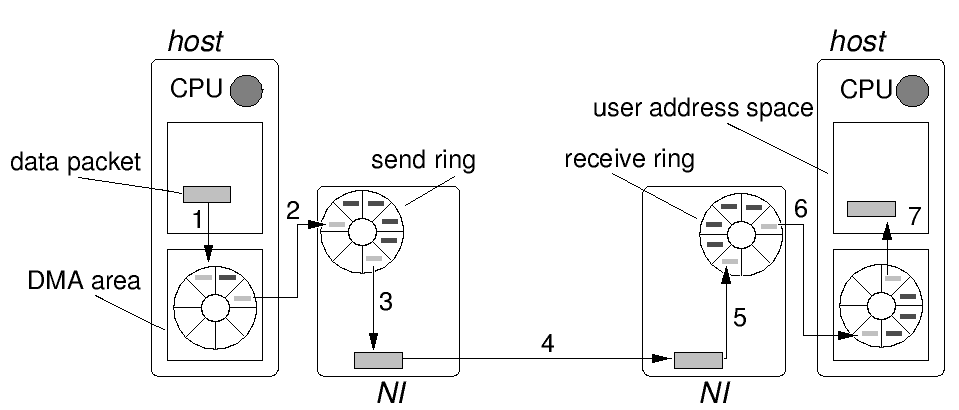
\includegraphics[width=\textwidth]{fig/overview.png} % overview.png: 1179666x1179666 pixel, 0dpi, infxinf cm, bb=
 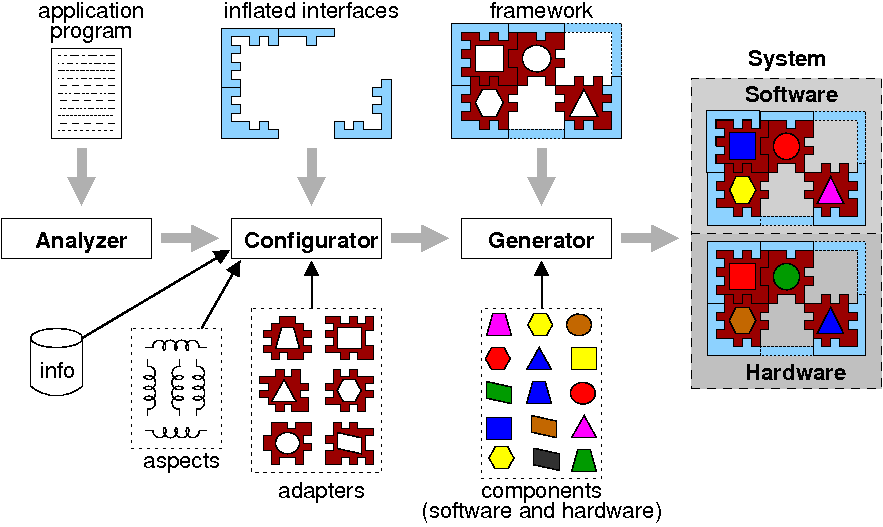
\includegraphics[width=12cm]{fig/overview5.png}
 \caption{An overview of the tool}
 \label{fig:overview}
\end{figure}



An application's source code, previously written based on the interfaces of components from a repository (the OS API), can be submitted to the \texttt{Analyzer} module. This module searches for references to the interfaces, identifying what features are necessary from each component, and elaborates a requirement specification that includes methods, types, and constants used by the application. If a requirement may be satisfied only by one component from the repository, the \texttt{Analyzer} can automatically choose it. If there are more than one, the components that meet the requirements, along with cost estimations, are presented to the developer so that he can choose the most adequate one.  The primary output of the \texttt{Analyzer} is a set of application dependencies, since the application depends on some components in order to work properly. These dependencies feed the \texttt{Configurator}.

The \texttt{Configurator} module is logically divided in a \texttt{Validator} and a \texttt{Configuration}. The components chosen with the help of the \texttt{Analyzer} are added to the \texttt{Configuration} and used by the \texttt{Validator} to build a dependency tree. By doing this, the \texttt{Validator} is able to keep track of (1) aplication dependencies, (2) component dependencies, and (3) component composition rules. (1) refers to the dependencies that exist between application requirements and system components. (2) refers to the dependencies that may exist between components and their traits and features. (3) refers to the rules that should be followed when creating the \texttt{Configuration}, since some component members may be exclusive, and critical components cannot be touched. Some components are critical to any configuration, while others are critical to specific target platforms.

Although the \texttt{Validator} leads the developer to choose only the components that are necessary and adequate, he can interact with the \texttt{Configurator} to add and remove components from the \texttt{Configuration} and modify their features and traits.

The last step in the system development process is accomplished by the \texttt{Generator} module. Internally, it works by generating a set of keys that represent the current valid \texttt{Configuration}, binding the interface used by the application to specific component members existent in the repository, and activating the scenario aspects eventually identified as necessary to satisfy the constraints dictated by the application or by the configured execution scenario. On the hardware side, the \texttt{Generator} produces a list of mediators that were included in the \texttt{Configuration}, specifying which ones are associated to IP blocks. These blocks are reusable hardware components, specified in a Hardware Description Language (HDL) or in an intermediate format, such as netlists.

The last step in the system development process is accomplished by the \texttt{Generator} module. Internally, it works by generating a set of keys that represent the current valid \texttt{Configuration}, binding the interface used by the application to specific component members existent in the repository, and activating the scenario aspects eventually identified as necessary to satisfy the constraints dictated by the application or by the configured execution scenario. On the hardware side, the \texttt{Generator} produces a list of mediators that were included in the \texttt{Configuration}, specifying which ones are associated to IP blocks, which are simple reusable hardware components, specified in a Hardware Description Language (HDL) or in an intermediate format, such as netlists.

%Note on 'key binding': The configuration keys mechanism binds the inflated interfaces of a family to the real implementation of one of their members.

The \texttt{Generator} module translates the keys into parameters for a statically metaprogrammed component framework and executes the compilation of a tailored system instance. In addition, whenever a SoC needs to be tailored, the \texttt{Generator} produces a synthesis configuration file that holds the parameters for configuring IP blocks and the information necessary to glue the IPs in a SoC. Written in a hardware description language, this configuration file and the selected IP blocks are handed over to a third-party tool, which performs the translation of the SoC specification into \textit{netlists}. Finally, by considering the target PLD technology, these netlists are translated into a configuration \textit{bitstream}.

%Note: A configuration is a collection of components that were selected from the repository to be included in the system instance, when generated.
%Note: A component belongs to a family of some type, and has at least one member. If a component is part of the configuration, at least one of its members must be selected.

%%%%%%%%%%%%%%%%%%%%%%%%%%%%%%%%%%%%%%%%%%%%%%%%%%%%%%%%%%%%%%%%%%%%%%%%%%%%%%%
\section{Prototype Implementation}
\label{sec:implementation}
%%%%%%%%%%%%%%%%%%%%%%%%%%%%%%%%%%%%%%%%%%%%%%%%%%%%%%%%%%%%%%%%%%%%%%%%%%%%%%%

A proof-of-concept Java implementation of the tool described in the previous section has been developed and some details of its operation at the current development stage are given here.

\subsection{Analyzer}

The \texttt{Analyzer} applies a technique that involves the compilation of the application's source code, a look at the resulting object files, and the identification of unresolved symbols that refer to methods and/or constants from the 'System' namespace. By doing this, it is able to identify the usage of the operating system API. The references to the API are extracted by an external Perl script and output in the form of a XML file. The file is used by the tool to generate application dependencies, and the subsequent suggestions of satisfactory components.

Figure~{\ref{fig:analyzer}} depicts the \texttt{Analyzer} GUI. This interface allows a developer to specify application implementation files and include directories containing header files, to visualize the code (right side), and to ask for requirements extraction. The requirements are exhibited in a tree structure (left side), which shows component families and members that satisfy the requirements. From the tree, the user may indicate the families and members to be included in the configuration.

We can observe a message console at the bottom of the figure. This console also accompanies the \texttt{Configurator} and \texttt{Generator} interfaces and shows all the relevant notifications, warnings, and error messages that must be delivered to the developer, relieving him from having to deal with dialog box windows.

\begin{figure}[ht!]
 \centering 
 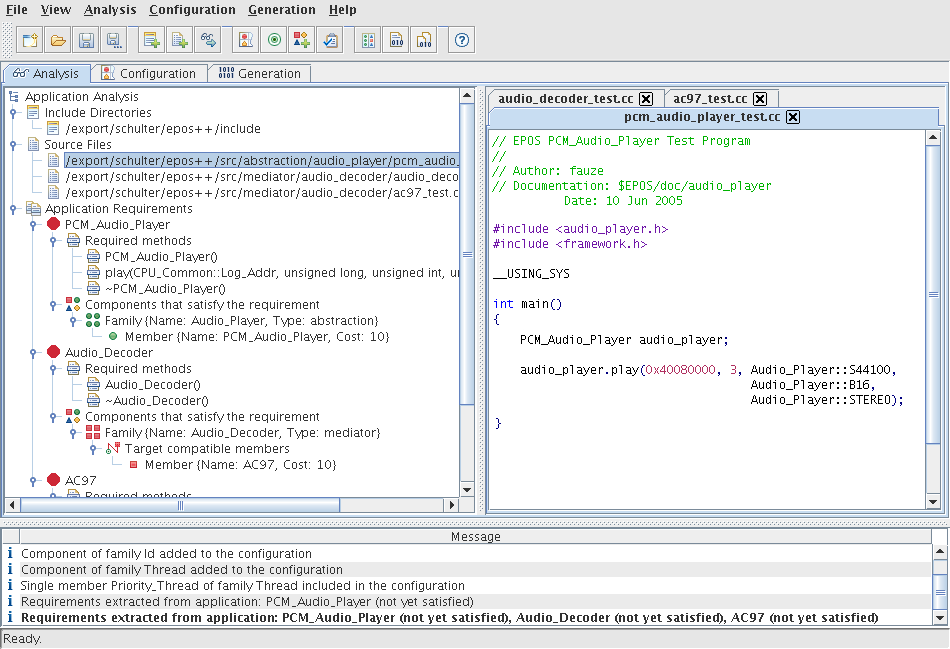
\includegraphics[width=\textwidth]{fig/analyzer.png} % analyzer.png: 1179666x1179666 pixel, 0dpi, infxinf cm, bb=
 \caption{The \texttt{Analyzer} interface}
 \label{fig:analyzer}
\end{figure}

\subsection{Configurator}
%HOW DOES THE REPOSITORY WORK?

The strategy used to describe components in a repository and their dependencies plays a key role in making the configuration process possible. The description must be complete enough so that the \texttt{Configurator} will be able to automatically identify which abstractions better satisfy the requirements of the application without generating conflicts or invalid configurations and compositions.

The component description language we adopted is based on XML and is focused on describing each component individually. As shown below, a component is defined by a \texttt{family} and its set of \texttt{member}. A family description also includes an \texttt{interface} declaration, an optional set of \texttt{dependency}, an optional set of \texttt{trait}, and a \texttt{common} package that holds \texttt{type} and \texttt{constant} declarations that are common to all family members.

\begin{mylisting}
\begin{verbatim}
<!ELEMENT family (interface, dependency*, trait*, common, member+)>
<!ELEMENT interface (type, constant, constructor, method)*>
<!ELEMENT common (type, constant)*>
<!ELEMENT member (super, interface, trait, cost, feature, dependency)*>
\end{verbatim}
\end{mylisting}

A family's interface summarizes the features of the whole family, including \texttt{constants}, \texttt{constructors}, and \texttt{methods}. Each member of a family is also described by an \texttt{interface}, which designates a total or partial realization of the family's interface. Additionally, a member is described by an optional \texttt{super} declaration, an optional set of \texttt{trait}, \texttt{dependency}, and \texttt{feature} declarations, and a required \texttt{cost} declaration.

The \texttt{super} element determines the inheritance from other members in the family, while a \texttt{trait} designates a configurable information that can be set by the developers, via the \texttt{Configurator}, in order to influence the instantiation of a component. A trait can also be used to specify configuration parameters that cannot be automatically figured out, such as the number of processors in a target machine or the amount of memory available.

The description of the interfaces in a family and its members is the main source of information for the \texttt{Configurator}, but correctly assembling a component-based system goes far beyond the verification of syntactic interface conformance: non-functional and behavioral properties must also be conveyed. For this purpose, the component description language includes two special elements: \texttt{feature} and \texttt{dependency}. These elements can be applied to virtually any other element in the language to specify features provided by components and dependencies among components that cannot be directly deduced from their interfaces. Enriching the description of components with features and dependencies can significantly improve the correctness of the assembly process, helping to avoid inconsistent component arrangements.

If the family is hardware mediator type or hardware IP type, the member descriptions must also declare \texttt{arch} and \texttt{mach}, which specify the architecture and machine the member is compatible with. More details and examples of the description language can be found in \cite{Tondello2004} \cite{Tondello2005}. 

%BAD FLOW HERE?
The \texttt{Configurator} GUI is depicted in Figure~{\ref{fig:configurator}}. It allows the developer to see the list of components included in the configuration (left side). Through the configuration desktop pane (right side), all the components, as well as the configuration's target platform, can be viewed and modified with the help of their respective configuration frames, although the default values for their features and traits are often adequate. The \texttt{Configurator} automatically includes the minimum necessary components and allows the developer to include other ones. However, currently it does not identify unnecessary or redundant components. Despite not being implemented, this could be achieved simply by analyzing the dependencies.

The \texttt{Validator} also has a graphical interface that opens up in the \texttt{Configurator} window. It shows the current collection of dependency problems and other miscellaneous ones, such as incorrect information describing component, target, or general configuration characteristics.

\begin{figure}[ht!]
 \centering 
 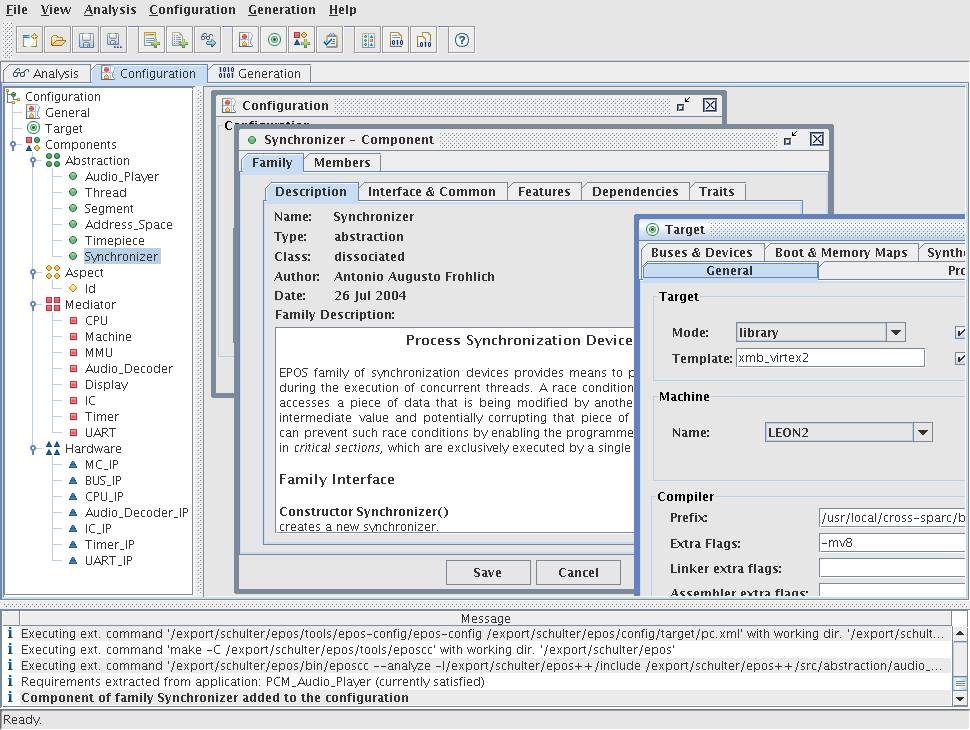
\includegraphics[width=\textwidth]{fig/configurator.png} % configurator.png: 1179666x1179666 pixel, 0dpi, infxinf cm, bb=
 \caption{The \texttt{Configurator} interface}
 \label{fig:configurator}
\end{figure}

\subsection{Generator}

The \texttt{Generator} allows a developer to launch processes that invoke the operating system's makefiles, causing the system instance generation, and processes that invoke synthesis tools that build the hardware platform. Before these generation processes can be executed, a set of directive files are created, including traits files and a 'keys file' that guide the generation. Also, the application may be compiled by the \texttt{Generator} with parameters that consider the system that was just built for it. Our approach aims at generating real systems, not only simulated ones. A limitation of this \texttt{Generator} is its inability to estimate properties (memory and silicon area, latency, power consumption, etc.) of the final system before really building it.

The \texttt{Generator} interface, as depicted in Figure~{\ref{fig:generator}}, is very straightforward. It shows informative output from the processes launched by their respective buttons. Some logic is applied to allow the actions a developer can take. For instance, it is not permitted to build the system or hardware before the 'Config' action is taken, since that action causes the generation of the directives needed by the building processes.

\begin{figure}[ht!]
 \centering 
 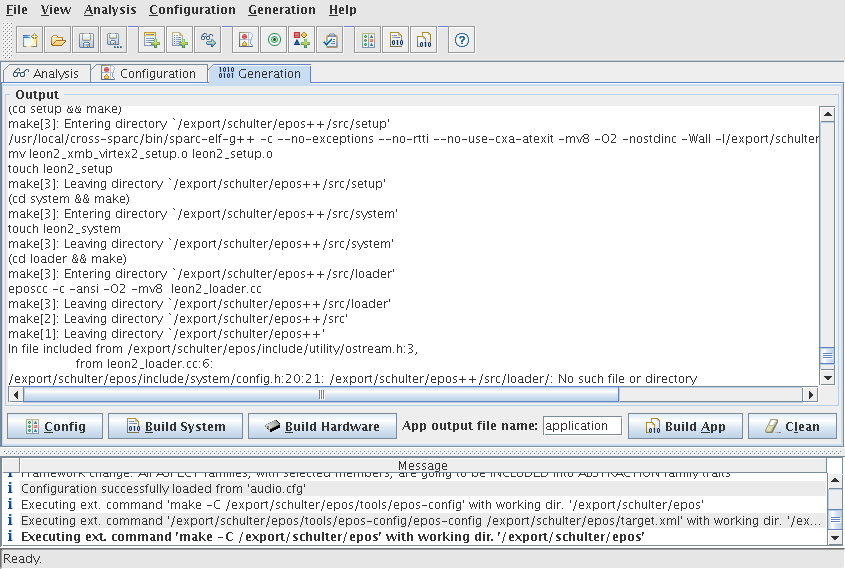
\includegraphics[width=\textwidth]{fig/generator.png} % generator.png: 1179666x1179666 pixel, 0dpi, infxinf cm, bb=
 \caption{The \texttt{Generator} interface}
 \label{fig:generator}
\end{figure}

This tool was designed to assist developers in executing the procedure depicted in Figure~{\ref{fig:overview}} in a simple, direct, and semi-automatic manner. The GUI and its usability have an important role, since it must greatly reduce the work a developer is required to do in comparison to what would be performed manually without tool assistance. Several conveniences, such as action keys, pop-up menus, icons, and intuitive responses are provided by it, and all the elements are organized in a way to make a clear separation of the activities related to analysis, configuration, and generation steps, although the developer is able to go back and forth through the steps. 

%%%%%%%%%%%%%%%%%%%%%%%%%%%%%%%%%%%%%%%%%%%%%%%%%%%%%%%%%%%%%%%%%%%%%%%%%%%%%%%
\section{Case Study and Results}
\label{sec:casestudy}
%%%%%%%%%%%%%%%%%%%%%%%%%%%%%%%%%%%%%%%%%%%%%%%%%%%%%%%%%%%%%%%%%%%%%%%%%%%%%%%

In order to evaluate the prototype implementation described in Section~{\ref{sec:implementation}} and its support for the requirements listed in Section~{\ref{sec:concepts}}, we performed some case studies involving the automatic or semi-automatic generation of different kinds of embedded applications, such as multimedia, automotive control, wireless sensor networks, energy aware mobile systems \cite{Hoellerjr2006} \cite{Wanner2006} for different platforms/architectures, such as AVR, MIPS, SparcV8, PPC405, and IA32.

In this paper we present a simple audio player application. The case study we will describe here was performed with the help of the EPOS component-based operating system and a Xilinx prototyping board as the target hardware platform. In order to avoid similar figures, all screenshots previously shown in this paper depict this case study.

%EPOS aims at delivering adequate run-time support for dedicated computing systems. An outcome of the AOSD method, EPOS consists of families of software components that can be adapted to fulfill the requirements of particular applications. Its component repository is a work a many years, and it supports a large array of hardware architectures, thus applications developed for EPOS are portable to several platforms.

The Xilinx board used as target contains a Virtex-II FPGA. Besides two built-in PowerPC 405 CPUs in that board (not used), a LEON2 soft-core processor was synthesized along with other IP blocks to create a system-on-a-chip. This board is targeted towards multimedia application prototyping and some of its available devices are: Memory Management Unit (MMU), Floating Point Unit (FPU), Time Stamp Counter (TSC), Interrupt Controller (IC), Data Service Unit (DSU), Watchdog, Universal Asynchronous Receiver/Transmitter (UART), Timer, Network Interface Card (NIC), Audio Decoder, Video Decoder, and Display Controller \cite{Pelgrims2003}. 

The application's source code is written in C++ and is listed below (the same that appears in Figure~{\ref{fig:analyzer}}). As we can see, only one method from the EPOS API is called, the \texttt{play(Log\_Addr sound, Seconds length, Sample\_Rate sample\_rate, Bit\_Depth bit\_depth, Sound\_Mode mode)} method from the \texttt{PCM\_Audio\_Player} abstraction. The parameters indicate that a \texttt{16-bit} \texttt{stereo} sound stream sampled at \texttt{44.1 khz} and stored at the \texttt{0x40080000} address should be played for \texttt{3} seconds.

\begin{mylisting}
\begin{verbatim}
// PCM_Audio_Player Test Program

#include <utility/ostream.h>
#include <audio_player.h>
#include <framework.h>

__USING_SYS

int main()
{
    PCM_Audio_Player audio_player;
    audio_player.play(0x40080000, 3, Audio_Player::S44100, Audio_Player::B16, Audio_Player::STEREO);
    return 0;
}
\end{verbatim}
\end{mylisting}
%http://www.kronto.org/thesis/tips/listings.html

The \texttt{PCM\_Audio\_Player} abstraction provides functionalities related to controlling the reproduction of uncompressed digital audio streams represented with Pulse Code Modulation (PCM). PCM is a standard for digital audio in computers and compact disks (CD) and is the usual output of audio decompressors, such as MPEG-1 Layer 3 (MP3) decoders.

The following is a description of the actions and interactions between a developer and the tool when the audio player application is submitted to begin the procedure:

\begin{itemize}
 \item The \texttt{Analyzer} identifies a reference to the \texttt{play()} method and suggests the \texttt{PCM\_Audio\_Player} abstraction component to satisfy this requirement. (see Figure~{\ref{fig:analyzer}})
 \item The developer interacts with the \texttt{Analyzer} and confirms that this component can be added to the \texttt{Configuration}.
 \item The \texttt{Configurator} acknowledges that the \texttt{PCM\_Audio\_Player} component is now an application dependency and adds it to the \texttt{Configuration}.
 \item The developer specifies that the target platform is a Virtex II Pro. (see Figure~{\ref{fig:configurator}})
 \item The \texttt{Validator} informs the developer that \texttt{PCM\_Audio\_Player} depends on the \texttt{Audio\_Decoder} mediator component.
 \item Among the \texttt{Audio\_Decoder} members, the \texttt{Configurator} suggests and automatically selects the \texttt{AC97} member, because it is the only mediator compatible with the target's architecture and available devices. The developer opts for maintaining the selection of this type of decoder.
 \item The \texttt{AC97} member from the \texttt{Audio\_Decoder} component depends on the \texttt{AC97} member from the \texttt{Audio\_Decoder\_IP} hardware component.
 \item The developer authorizes the inclusion of the \texttt{Audio\_Decoder\_IP} component and its \texttt{AC97} member is automatically selected.
 \item Besides these player and decoder components, three critical components are automatically included by the \texttt{Configurator} and cannot be removed: \texttt{CPU}, \texttt{Machine}, and \texttt{Thread}. The \texttt{CPU} component is the most critical. The \texttt{Machine} component mediates the platform architecture and is automatically configured with trait values (architecture, processor, memory, etc.) that conform to the target the developer has previously chosen. The \texttt{CPU} and \texttt{Machine} are hardware mediators and, because of this, need to be compatible with the target's architecture. The \texttt{Configurator} automatically selects their members based on this requisite. Finally, the \texttt{Thread} component is included to support the runtime of the application, even though it is not multi-threaded.
 \item When the developer finishes interacting with the \texttt{Configurator} to solve the dependencies that have appeared, the \texttt{Validator} allows the generation process to occur.
 \item The developer pushes some of the \texttt{Generator} buttons, causing the system generation. This consists of compiling the highly customized instance of EPOS, calling the \textit{Xilinx Synthesis Tool} (XST) to build the hardware, compiling the application, and linking the resulting object files to create a bootable image. This image is a few kilo bytes in size and is ready to be uploaded to the hardware's memory and tested (see Figure~{\ref{fig:generator}}).
\end{itemize}

Figure~{\ref{fig:casestudy}} depicts the components included in this case study's configuration and the dependencies existent between them. %note: some dependencies that appear in the diagram are not explained, on purpose

\begin{figure}[ht!]
 \centering 
 %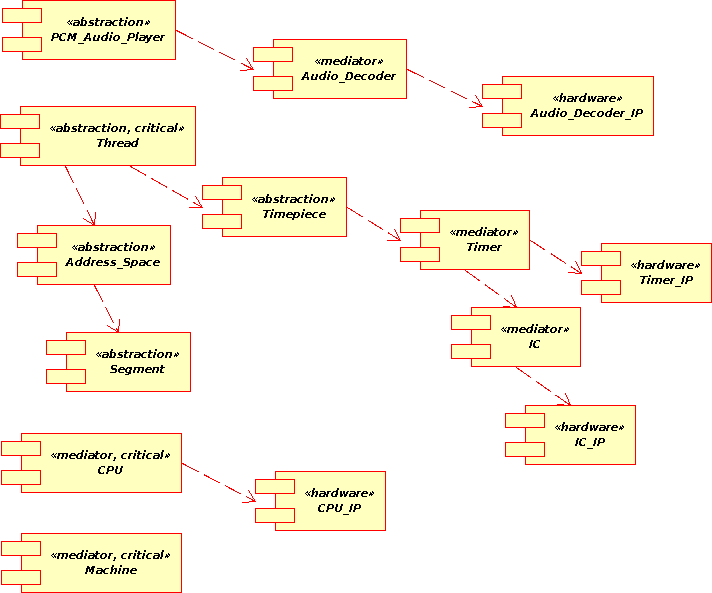
\includegraphics[width=\textwidth]{fig/casestudy.png} % casestudy.png: 1179666x1179666 pixel, 0dpi, infxinf cm, bb=
 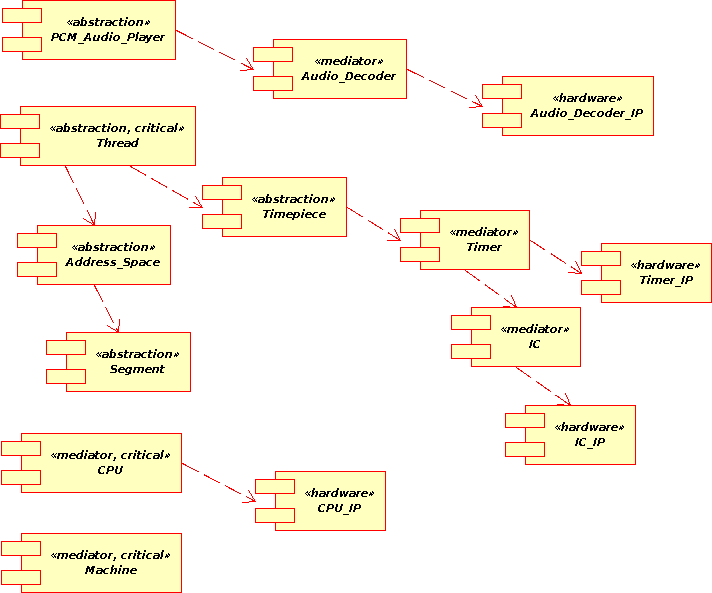
\includegraphics[width=10cm]{fig/casestudy.png} % casestudy.png: 1179666x1179666 pixel, 0dpi, infxinf cm, bb=
 \caption{Component diagram of the audio player system configuration}
 \label{fig:casestudy}
\end{figure}

We found that this tool is adequate for the use case described here, since it satisfies the requirements elicited in Section~{\ref{sec:concepts}}: application analysis; component suggestions, component selection, configuration, and composition; generation of system software and hardware; configuration validation; specific graphical interface; feedback to the developer; and partial automation. Cost estimations, though, is a requirement that currently is not fully supported, since no meaningful estimations for each of the components are calculated.

Several other applications, components, and target platforms were tested with the tool. Its strong points are its fast and simple operation and its internal design that features good maintainability and extensibility. Another aspect to consider is the possibility of using it to configure and generate other component-based operating systems. This would be possible if such systems provide some of the facilities EPOS does: a component repository properly described in a language the tool knows how to interpret and a set of makefiles that provide building rules.

%Some of the limitations, along with possible solutions, are listed below:
%
%\begin{itemize}
% \item The tool does not identify unnecessary or redundant components: this could be achieved by analyzing the dependencies.
% \item The \texttt{Configurator} is not as automatic as it could be: could be improved if it tried to automatically solve some dependencies by considering cost estimations and project goals, such as real-time operation or energy efficiency.
% \item The repository cannot be manipulated from inside the tool: this is a desirable feature that would facilitate the creation, removal, and modification of component implementations. The creation of new components would be facilitated if the tool generated partially implemented header and source files based on the interfaces specificed by the component developer.
% \item The tool does not estimate the system image size before its generation: this would be useful to improve the development speed when the target platform's memory has restricted size.
%\end{itemize}

%%%%%%%%%%%%%%%%%%%%%%%%%%%%%%%%%%%%%%%%%%%%%%%%%%%%%%%%%%%%%%%%%%%%%%%%%%%%%%%
\section{Conclusions}
%%%%%%%%%%%%%%%%%%%%%%%%%%%%%%%%%%%%%%%%%%%%%%%%%%%%%%%%%%%%%%%%%%%%%%%%%%%%%%%

In this paper we dealt with the problem of developing embedded systems. Even with component-based design, current solutions do not address efficiently architectural transparency, performance, configuration and generation of application oriented embedded systems. We have shown the basic concepts of Application-Oriented System Design methodology that was developed to solve these problems and we focused here on the final phase of development.

We have presented a tool that assists developers in configuring and generating software and hardware support for embedded systems taking as base a collection of reusable components developed according with the Application-Oriented System Design methodology, their dependencies and composition rules. The prototype implements the requirements listed in Section \ref{sec:concepts}, and effectively identifies, selects, configures, adapts, and composes those components, generating real and functional embedded systems. Steps are performed automatically whenever possible by the current prototype and some hints are given when design decisions are required. The developer can focus on his application, not on the underlying support system, which leads to a faster development process and, incidentally, shorter time-to-market for commercial products.

As a case study, an example of a configuration process for a simple but real application was presented, as well as the current limitations of the model due to the need of manual selection when more than one different component satisfy the required interface. We believe that it represents an important step in the direction of a fully automated generation since we have promoted the generation of software and hardware support and SoC instances in the same generation flow according to a well defined methodology. The strategy currently realized does not represent a complete solution to automate the process of generating SoC-based embedded systems (whereas the programmer still takes some decisions regarding the selection of more than one different realization for a component). We believe a more detailed costs model for components and the inclusion of a smarter algorithm to perform design exploration could automatically solve most of the situations. However, some decisions will seldom be fully automatic, such as choosing the best real-time scheduler component that garantees deadlines will be meet based only on application source code and on component interfaces.

The components existent in our repository were identified and defined with the AOSD approach, which starts with domain analysis, identification of families, identification of members and aspects. Since great attention is required when performing these steps, the actual specification of components and their features does not require much effort. A developer needs only to implement their code and add some lines of description in configuration rules files. The maintainance of these components is also not a hard task, since abstraction components will seldom be modified, and hardware mediator ones have different implementations for each platform they refer to.

Our road map for future work includes simple improvements, such as the implementation of a convenient GUI that shows numbers and charts that better represent the system, to make the \texttt{Configurator} responsible for finding out if there are any unnecessary, redundant, or not very adequate components, to include convenient repository manipulation functionalities to help developer in managing component implementations, and to provide a simple source code editor for the \texttt{Analyzer}.

Finally, the results obtained with Application-Oriented System Design, the EPOS framework, and the tool described in this paper are so far encouraging. Research in progress is looking forward to improve the costs model for components and allow intelligent design space exploration for automatic and adaptive component selection and partitioning. With this, our approach would not only automatically generate systems that match applications requirements, but also design requirements, such as as maximum silicon area or power consumption.


%---------------------------------------------------------------------
% BIBLIOGRAPHY
%---------------------------------------------------------------------
%\begin{thebibliography}{XXXXX}
%\bibitem[]{}
%\end{thebibliography}

\bibliographystyle{plain}
\bibliography{tools2007}


%---------------------------------------------------------------------
% ABOUT THE AUTHORS
%---------------------------------------------------------------------

% This command starts the ``About the Authors'' section.
\abouttheauthors

\abouttheauthor[alexandre]{Alexandre Schulter}{works as an IT analyst at Dataprev, a brazillian public company. In the past he has worked as a researcher and software developer at several laboratories in the Technological Centre, Federal University of Santa Catarina, Brazil. He holds the MSc (2006) and Bachelor (2003) degrees in Computer Sciences, and his areas of interest include Information Systems, Component-based Systems, Computer-Aided Software Engineering, Distributed Systems, Grid Computing, and Security.
\maillink{schulter@inf.ufsc.br}. 
See also \htmllink{http://www.inf.ufsc.br/\~{}schulter}.}

\abouttheauthor[cancian]{Rafael Luiz Cancian}{is a PhD canditate in Electrical Engineering at the Federal University of Santa Catarina, Master (2000) and Bachelor (1997) in Computer Sciences at the Federal University of Santa Catarina (UFSC). Currently he is a professor of the Computer Sciences Department at University of Vale do Itaja\'i - UNIVALI (Itaja\'i, Brazil), and associated researcher of the Laboratoty of Software and Hardware Integration (LISHA/UFSC) and the Laboratory of Embedded and Distributed Systems (LSED/UNIVALI).
\maillink{cancian@das.ufsc.br}. 
See also \htmllink{http://www.das.ufsc.br/\~{}cancian}.}

% Graduação: Engenharia Elétrica (1978-1982) pela UFSC.
% Mestrado: Sistemas de Controle, Automação e Informática Industrial (1983-1985) pelo LCMI/UFSC. Título da Dissertação: "Projeto e Implementação de um Monitor Multitarefas em Tempo Real". Orientador: Prof. Dr.-Ing. Jean-Marie Farines.
% Doutorado: Automação Industrial, Redes Industriais (1986-1991) pelo WZL / RWTH-Aachen, Alemanha. Título da Tese: "Einsatzmöglichkeiten digitaler Feldbussysteme in geschlossenen, maschineninternen Regelkreisen" (Possibilidades de Aplicação de Redes Fieldbus em Malhas Fechadas de Controle Intramáquina). Orientador: Prof. Dr.-Ing. Dr. h. c. Tilo Pfeifer.
% Estágio de Pós-Doutorado: Reconhecimento de Padrões (2004-2005) no LIP6 / UPMC (Paris VI), França. Anfitrião: Prof. Dr. Patrick Gallinari.
% Atividade Atual: coordenador do grupo de pesquisa S2i e Professor Adjunto IV do Departamento de Automação e Sistemas (DAS) da Universidade Federal de Santa Catarina (UFSC).
\abouttheauthor[marcelo]{Marcelo Ricardo Stemmer}{is a PhD in Industrial Automation (1991) (WZL / RWTH-Aachen, Germany), Master (1985) and Bachelor (1982) in Electrical Engineering (1985) (Federal University of Santa Catarina - UFSC). Currently he is a professor at the Department of Automation and Systems (DAS) of the Federal University of Santa Catarina (Florian\'opolis, Brazil), and head of the Intelligent Industrial Systems (S2i) research group at UFSC.
\maillink{marcelo@das.ufsc.br}. 
See also \htmllink{http://www.das.ufsc.br/\~{}marcelo}.}

%Antônio Augusto Medeiros Fröhlich possui doutorado em Engenharia da Computação pela Universidade Técnica de Berlim, Mestrado em Ciência da Computação pela Universidade Federal de Santa Catarina e graduação em Ciência da Computação pela Universidade Federal do Rio Grande do Sul. Atualmente é professor do Departamento de Informática e Estatística (INE) e do Programa de Pós-Graduação em Ciência da Computação (PPGCC) da Universidade Federal de Santa Catarina (UFSC), onde coordena também o Laboratório de Integração de Software e Hardware (LISHA). O Prof. Fröhlich é autor de um livro e de uma série de artigos na área de sistemas operacionais e sistemas embarcados, áreas nas quais coordena e executa uma série de projetos de pesquisa e desenvolvimento.
\abouttheauthor[guto]{Ant\^{o}nio Augusto Medeiros Fr\"{o}hlich}{is a PhD in Computer Engineering (Technical University of Berlin), MSc in Computer Science (Federal University of Santa Catarina), and Bachelor in Computer Science (Federal University of Rio Grande do Sul). Currently he is an associate professor at the Computer Science Department of the Federal University of Santa Catarina (Florian\'opolis, Brazil), head of the Laboratory for Software/Hardware Integration (LISHA) at Federal University of Santa Catarina, and external research associate at the Fraunhofer FIRST within the Software Engineering Group (Berlin, Germany).
 
\maillink{guto@lisha.ufsc.br}. 
See also \htmllink{http://www.lisha.ufsc.br/\~{}guto}.}



%---------------------------------------------------------------------
\end{document}
%---------------------------------------------------------------------
